%% Adapted from GaTech CS 7545 Machine Learning Theory given by Prof. Jacob Abernathy Fall 2018. Original latex file: https://github.com/mltheory/CS7545/blob/master/scribe/CS7545scribe_template.tex 



%%%%%PLEASE CONSIDER CORRECTIONS AT PLACES INDICATED%%%%%%%%
\documentclass{article}
%%%%%Packages Used, add more if necessary%%%%
\usepackage{amsmath,amsfonts,amssymb,graphicx,fullpage}
\setlength{\topmargin}{-0.6 in}
\setlength{\textheight}{8.5 in}
\setlength{\headsep}{0.75 in}
\usepackage{mdframed}
\usepackage{multicol}
\usepackage{microtype}
\usepackage{float}
\usepackage{subcaption}
\usepackage{hyperref}
\usepackage{cite}
\newcommand{\vecb}[1]{\boldsymbol{#1}} % bold Greek / symbols
\newcommand{\matb}[1]{\mathbf{#1}}     % bold matrices
\newcommand{\vb}[1]{\mathbf{#1}}       % bold vectors (latin)

%%%%% NO NEED TO EDIT THIS PREAMBLE %%%%%%%%
%%% PREAMBLE %%%
\newcounter{lecnum}
\renewcommand{\thepage}{\thelecnum-\arabic{page}}
\renewcommand{\thesection}{\thelecnum.\arabic{section}}
\renewcommand{\theequation}{\thelecnum.\arabic{equation}}
\renewcommand{\thefigure}{\thelecnum.\arabic{figure}}
\renewcommand{\thetable}{\thelecnum.\arabic{table}}
\newcommand{\lecture}[4]{
   \pagestyle{myheadings}
   \thispagestyle{plain}
   \newpage
   \setcounter{lecnum}{#1}
   \setcounter{page}{1}
   \noindent
   \begin{center}
   \framebox{
      \vbox{\vspace{2mm}
      
      \hbox to 6.28in { 
      {\bf ECE 4252/6252 (FunML) Fundamentals of Machine Learning \hfill 2021--2028} }
      
      \vspace{2mm}
      \hbox to 6.28in { 
      {Courses developed by Professor Ghassan AlRegib 
      (\href{https://alregib.ece.gatech.edu/}{alregib.ece.gatech.edu}) 
      \hfill For inquiries: \href{mailto:alregib@gatech.edu}{alregib@gatech.edu}} }
      
      \vspace{3mm}
      \hbox to 6.28in { {\Large \hfill Lecture #1: #2 \hfill} }
      
      \vspace{2mm}
      \hbox to 6.28in { {\it Co-Instructors: #3 \hfill #4} }
      
      \vspace{2mm}}
   }
   \end{center}

   % -------- PEOPLE OUTSIDE BOX --------
   \vspace{2mm}
   \noindent{\bf Contributors:} Dr. Ahmad Mustafa, Dr. Motaz Alfarraj, Dr. Ashraf Alattar, Dr. Chen Zhou

   \vspace{1mm}
   \noindent{\bf Teaching Assistants} with remarkable contributions include: Kuo-Wei Lai, Wuyang Du, Shiva Mahato, Michael Zhou, Ninghan Zhong

   \markboth{Lecture #1: #2}{Lecture #1: #2}

   \vspace{2mm}
\noindent {\bf Disclaimer}: 
{All content of these notes are part of this course at Georgia Tech. Any re-use or distribution is not permitted without pre-approved permission. All these notes belong to, created by, and copyrighted for Ghassan AlRegib and Mohit Prabhushankar, Georgia Tech, 2021--2028.}



\vspace{2mm}
\noindent {\bf License}: 
{These lecture notes are licensed under the 
\href{https://creativecommons.org/licenses/by-nc-sa/4.0/}{Creative Commons Attribution-NonCommercial-ShareAlike 4.0 International License}.}

   \vspace{2mm}
   \noindent {\bf Errata}: 
   {\it Please submit any errata you find using the following form: 
   \href{https://forms.office.com/r/fbg9dMWPgY}{Errata Form for FunML Textbook} 
   or visit: \url{https://forms.office.com/r/fbg9dMWPgY}}

   \vspace*{4mm}
}
% \renewcommand{\cite}[1]{[#1]}
% \def\beginrefs{\begin{list}
%         {[\arabic{equation}]}{\usecounter{equation}
%          \setlength{\leftmargin}{2.0truecm}\setlength{\labelsep}{0.4truecm}%
%          \setlength{\labelwidth}{1.6truecm}}}
% \def\endrefs{\end{list}}
% \def\bibentry#1{\item[\hbox{[#1]}]}

\newcommand{\challenge}[2]{\noindent \textbf{(Challenge Problem)} \emph{#1}: #2 }

\newcommand{\exercise}[1]{\noindent \textbf{(Exercise)} #1 }

\newcommand{\fig}[3]{
			\vspace{#2}
			\begin{center}
			Figure \thelecnum.#1:~#3
			\end{center}
	}
%%% END_OF_PREAMBLE %%%


	
%%%%You may add more \newtheorem if necessary%%%%%%
\newtheorem{theorem}{Theorem}[lecnum]
\newtheorem{lemma}[theorem]{Lemma}
\newtheorem{proposition}[theorem]{Proposition}
\newtheorem{claim}[theorem]{Claim}
\newtheorem{corollary}[theorem]{Corollary}
\newtheorem{definition}[theorem]{Definition}
\newenvironment{proof}{{\bf Proof:}}{\hfill\rule{2mm}{2mm}}


\newcommand{\dom}{\mathrm{dom}}
\begin{document}

\lecture{9}{Second-Order Optimization Methods}{Ghassan AlRegib and Mohit Prabhushankar}{}%

\section{Recap and Lecture Objectives}

In the previous lecture, we continued our study of regression models and the key tools used to train and evaluate them. We covered optimization methods for fitting regression models, including gradient-based approaches as well as \textbf{Newton’s Method} and \textbf{Coordinate Search}. We also discussed how \textbf{regularization} improves generalization in linear regression, with particular emphasis on \textbf{Ridge} and \textbf{Lasso}, and we reviewed common performance measures such as Mean Squared Error (MSE), Mean Absolute Error (MAE), and the Coefficient of Determination ($R^2$).

In this lecture, we build on those foundations by organizing the regression workflow end-to-end. We begin by summarizing optimization methods beyond basic gradient descent, including \textbf{Newton’s Method} (which uses curvature through the Hessian) and \textbf{coordinate-based methods} such as Coordinate Search and Coordinate Descent. Next, we revisit \textbf{regularization}—including Ridge ($\ell_2$), Lasso ($\ell_1$), and Elastic Net—to understand how controlling coefficient magnitudes helps prevent overfitting. We then review key \textbf{performance metrics} for regression, including MSE, RMSE, MAE, and $R^2$.

Finally, the main focus of this lecture is \textbf{model validation and evaluation}. We introduce the train/validation/test split, learning curves, cross-validation, and the bias--variance tradeoff, which together provide a practical framework for understanding model generalization and performance on unseen data. We also highlight how evaluation becomes more subtle when labels are noisy or ambiguous.



\section{Second-Order Optimization: Newton's Method}

Second-order optimization methods improve upon Gradient Descent by using curvature information of the loss surface. Instead of relying only on the slope (first derivative), these methods also use second derivatives to better estimate the location of the minimum.

\subsection{Jacobian and Hessian Matrices}

The Jacobian matrix is a matrix composed of first-order partial derivatives of a multivariable function. It describes how a function changes with respect to each variable and is commonly used in optimization and nonlinear systems. The Hessian matrix extends this idea by collecting second-order partial derivatives. It is an \( n \times n \) square matrix that captures the curvature of a function and plays a central role in second-order optimization methods.

For example, consider the function \( f(x,y) = x^2y + y^2x \). The Hessian matrix for this function is
\[
H_f(x,y)=
\begin{pmatrix}
2y & 2x+2y\\
2x+2y & 2x
\end{pmatrix}.
\]

\subsection{Optimization}

Second-order optimization methods use curvature information to guide the search for a minimum. While first-order methods such as Gradient Descent rely only on the slope of the loss surface, second-order methods additionally use the Hessian matrix to capture how the surface bends. This curvature information allows the optimizer to take more informed steps toward the minimum.

When the Hessian matrix is positive semi-definite,
\[
\Delta\vecb{\theta}^T \matb{H}(\vecb{\theta})\Delta\vecb{\theta} \ge 0
\quad \text{for any } \Delta\vecb{\theta}.
\]
the loss surface locally behaves like a convex parabola. In this setting, curvature information can be used to construct a more accurate local model of the loss function.

Using a second-order Taylor approximation, the loss near a point \( \vecb{\theta} \) can be written as
\[
L(\vecb{\theta}+\Delta\vecb{\theta})
\approx
L(\vecb{\theta})
+\Delta\vecb{\theta}^T\nabla_{\vecb{\theta}} L(\vecb{\theta})
+\frac{1}{2}\Delta\vecb{\theta}^T \matb{H}(\vecb{\theta})\Delta\vecb{\theta}.
\]
To find the minimum of this quadratic approximation, we set the derivative with respect to \( \Delta\theta \) equal to zero:
\[
\nabla_{\vecb{\theta}} L(\vecb{\theta})
+\matb{H}(\vecb{\theta})\Delta\vecb{\theta}=0,
\]

which yields the optimal update direction
\[
\Delta\vecb{\theta}
=
-\matb{H}(\vecb{\theta})^{-1}
\nabla_{\vecb{\theta}} L(\vecb{\theta}).
\]

Substituting this update into the iterative optimization framework leads to the Newton’s Method update rule
\[
\vecb{\theta}^{t+1}
=
\vecb{\theta}^{t}
-\alpha \matb{H}(\vecb{\theta})^{-1}
\nabla_{\vecb{\theta}} L(\vecb{\theta}).
\]

For comparison, standard Gradient Descent uses only first-order information:
\[
\vecb{\theta}^{t+1}
=
\vecb{\theta}^{t}
-\alpha \nabla_{\vecb{\theta}} L(\vecb{\theta}^{t}).
\]


A matrix is positive semi-definite when it is symmetric and has non-negative eigenvalues, which guarantees locally convex curvature and enables reliable descent toward a minimum.

\begin{figure}[H]
    \centering
    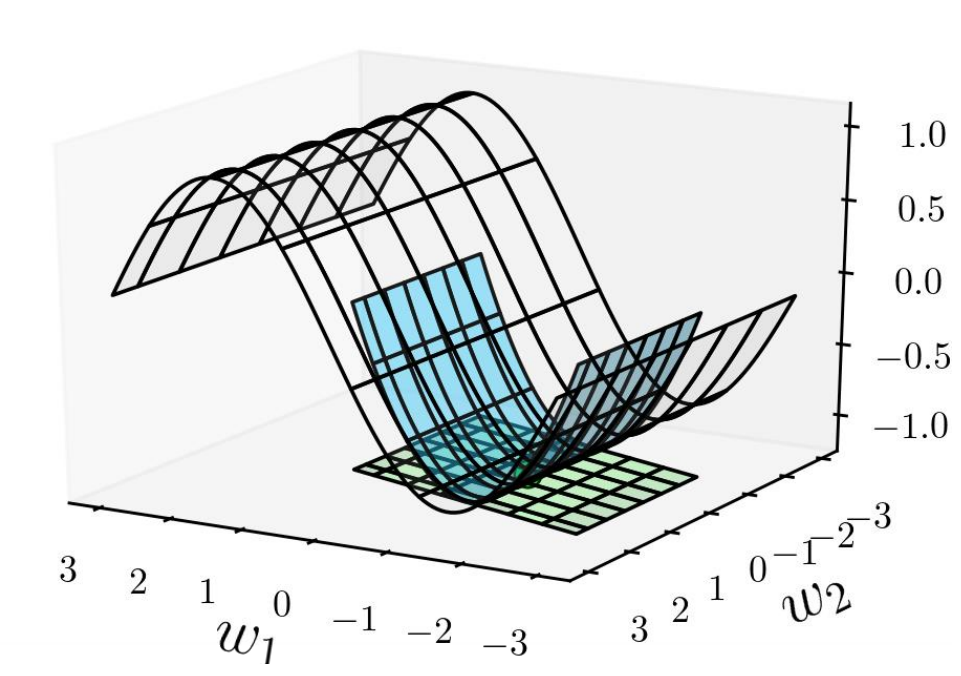
\includegraphics[width=0.4\textwidth]{img/lecture9/P2.png}
    \caption{Figure 9.1: Visualization of the function with respect to parameters \(w_1\) and \(w_2\) (quadratic function in blue)}
    \label{fig:P2.png}
\end{figure}


\subsection{Convexity}

In optimization, the concept of convexity plays a crucial role in determining how easily we can find the global minimum of a function. A function \( f(\vecb{\theta}) \) is said to be \textit{convex} if, for any two points \( \vecb{\theta}_1 \) and \( \vecb{\theta}_2 \) within its domain, the line segment connecting \( f(\theta_1) \) and \( f(\theta_2) \) lies above or on the graph of the function itself. Formally, for any \( \vecb{\theta}_1, \vecb{\theta}_2 \in \mathrm{dom}(f) \) and \( \lambda \in [0,1] \):
\[
f(\lambda \vecb{\theta}_1 + (1-\lambda) \vecb{\theta}_2)
\leq \lambda f(\vecb{\theta}_1) + (1-\lambda) f(\vecb{\theta}_2).
\]

This property guarantees that the function has a single global minimum and no other local minima, making optimization significantly easier.

For twice-differentiable functions, convexity can be checked using the Hessian matrix. A function is convex if its Hessian is positive semi-definite everywhere:
\[
\matb{H}(\vecb{\theta}) \succeq 0.
\]
This means the loss surface curves upward in every direction, forming a bowl-shaped landscape that guides optimization algorithms toward the global minimum.

In contrast, \textit{non-convex} functions do not satisfy the convexity condition. The line segment between two points may lie below the function curve, producing multiple local minima and maxima. In these cases, optimization algorithms such as gradient descent may become trapped in local minima and fail to reach the global solution.


\subsection{Convergence}

Newton's method is particularly powerful for minimizing \textit{convex} functions. Because it incorporates curvature information through the Hessian, it produces a quadratic approximation of the loss surface at every step. This allows the algorithm to move directly toward the minimum rather than following the slower zig-zag path typical of gradient descent.

Near the optimum, Newton’s method exhibits \textbf{quadratic convergence}, meaning the error decreases extremely rapidly once the algorithm is close to the minimum. In contrast, gradient descent typically achieves only \textbf{linear convergence}, requiring many more iterations to reach a similar level of accuracy.

However, Newton's method becomes less reliable for \textit{non-convex} functions. When the Hessian is not positive semi-definite, the quadratic approximation may point toward a saddle point or even a local maximum. As illustrated in the figures, the method may converge to an undesirable local minimum, move toward a local maximum, or oscillate between regions due to incorrect curvature information. 

For this reason, Newton’s method is most effective when the loss function is convex or when the optimization has already reached a region close to a local minimum.


\begin{figure}[H]
    \centering
    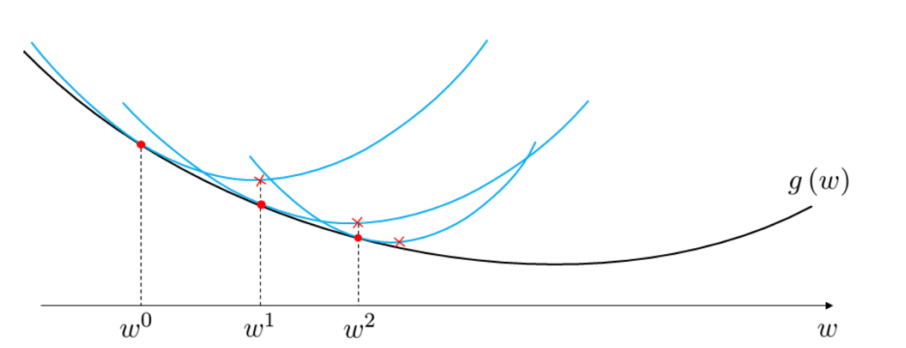
\includegraphics[width=0.4\textwidth]{img/lecture9/P3.png}
    \caption{Figure 9.2: Newton's Method Convergence: Convex Functions}
    \label{fig:P3.png}
\end{figure}

\begin{figure}[H]
    \centering
    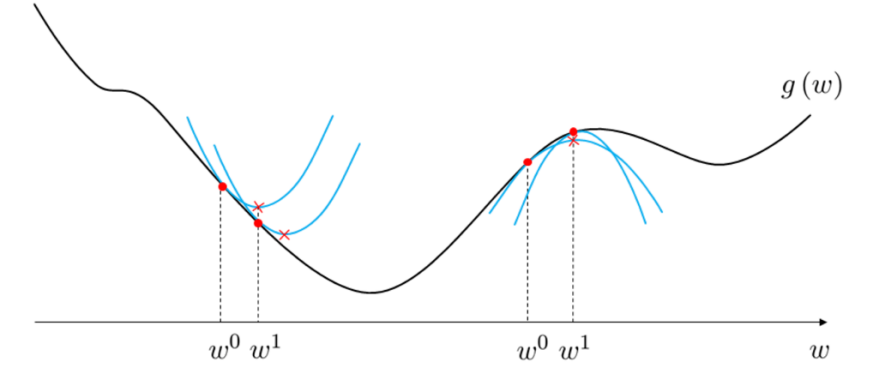
\includegraphics[width=0.4\textwidth]{img/lecture9/P4.png}
    \caption{Figure 9.3: Newton's Method Convergence: Non-Convex Functions}
    \label{fig:P4.png}
\end{figure}


\subsection{Computational Complexity}

Although Newton’s method can converge in fewer iterations than first-order methods, it is significantly more expensive per iteration. The main challenge is the Hessian matrix, which is a \(P \times P\) matrix containing all second-order partial derivatives of the loss function.

Storing the Hessian requires \(O(P^2)\) memory, which quickly becomes impractical for models with many parameters. Computing the Hessian itself requires \(O(P^2)\) operations, and computing its inverse requires approximately \(O(P^3)\) time. Therefore, the total computational cost per Newton update is dominated by the matrix inversion step:

\[
\vecb{\theta}^{t+1}
=
\vecb{\theta}^{t}
-\alpha \matb{H}(\vecb{\theta})^{-1}
\nabla_{\vecb{\theta}} L(\vecb{\theta})
\]

Where \(\matb{H}(\vecb{\theta})\) is the Hessian matrix:
\[
\matb{H}(\vecb{\theta})=\nabla_{\vecb{\theta}}^2 L(\vecb{\theta})
\]

\[
\boxed{\textbf{Total time per iteration of Newton's Method: } O(P^3)}
\]

Because modern machine learning models often contain millions of parameters, directly computing and inverting the Hessian is typically infeasible. For this reason, most large-scale learning algorithms rely on first-order methods such as Gradient Descent or use approximate second-order methods (e.g., quasi-Newton methods) that avoid explicit Hessian computation.



% \subsection{Newton’s Method: Second-order Taylor Approximation}

% Newton’s method is a local optimization technique that uses a second-order Taylor series approximation of the loss function to obtain a more accurate estimate of the direction toward the minimum. Instead of relying only on the gradient, this approach incorporates curvature information through second-order derivatives, leading to faster convergence near an optimum.

% Using a second-order Taylor expansion, the loss function around the current parameter vector can be approximated as
% \[
% L(\theta + \Delta \theta) \approx L(\theta) + \Delta \theta^T \nabla_\theta L(\theta) + \frac{1}{2} \Delta \theta^T H(\theta) \Delta \theta .
% \]
% Here, \(\nabla_\theta L(\theta)\) denotes the gradient of the loss function, while \(H(\theta)=\nabla_\theta^2 L(\theta)\) is the Hessian matrix, which contains all second-order partial derivatives:
% \[
% H(\theta)=
% \begin{pmatrix}
% \frac{\partial^2 L(\theta)}{\partial \theta_1^2} & \cdots & \frac{\partial^2 L(\theta)}{\partial \theta_1 \partial \theta_p} \\
% \vdots & \ddots & \vdots \\
% \frac{\partial^2 L(\theta)}{\partial \theta_p \partial \theta_1} & \cdots & \frac{\partial^2 L(\theta)}{\partial \theta_p^2}
% \end{pmatrix}.
% \]

% This formulation assumes that the loss function is twice differentiable so that the Hessian exists. The resulting quadratic approximation provides a more accurate local model of the loss surface than first-order methods alone, allowing Newton’s method to move toward the minimum more efficiently, particularly when the optimization is close to convergence.



\section{Coordinate Search}

When gradient information is unavailable or too expensive to compute, derivative-free optimization methods provide an alternative strategy.

\subsection{Optimization}

Coordinate search is a simple optimization technique that does not rely on gradients or second-order derivatives. Instead of computing the steepest descent direction, the algorithm explores the parameter space by moving along one coordinate axis at a time. At each iteration, the method tests whether moving in the positive or negative direction of a coordinate decreases the loss, and updates the parameters accordingly. The update rule is

\[
\vecb{\theta}^{t+1}
=
\vecb{\theta}^{t}
\pm \alpha \vb{e}_j
\]


where \(\vb{e}_j = [0, \ldots, 1, \ldots, 0]^T\) is the \(j\)-th standard basis vector, which selects the coordinate direction being explored.

This approach is useful when gradients are unavailable, difficult to compute, or expensive to evaluate. Because it does not require derivatives, coordinate search belongs to the class of \textit{derivative-free optimization} methods. However, this simplicity comes at a cost: the algorithm may require many function evaluations and can be slower than gradient-based methods in high-dimensional problems.

Figure~\ref{fig:P5.png} illustrates how the algorithm explores descent directions along coordinate axes, moving step-by-step toward lower values of the objective function.

\begin{figure}[H]
    \centering
    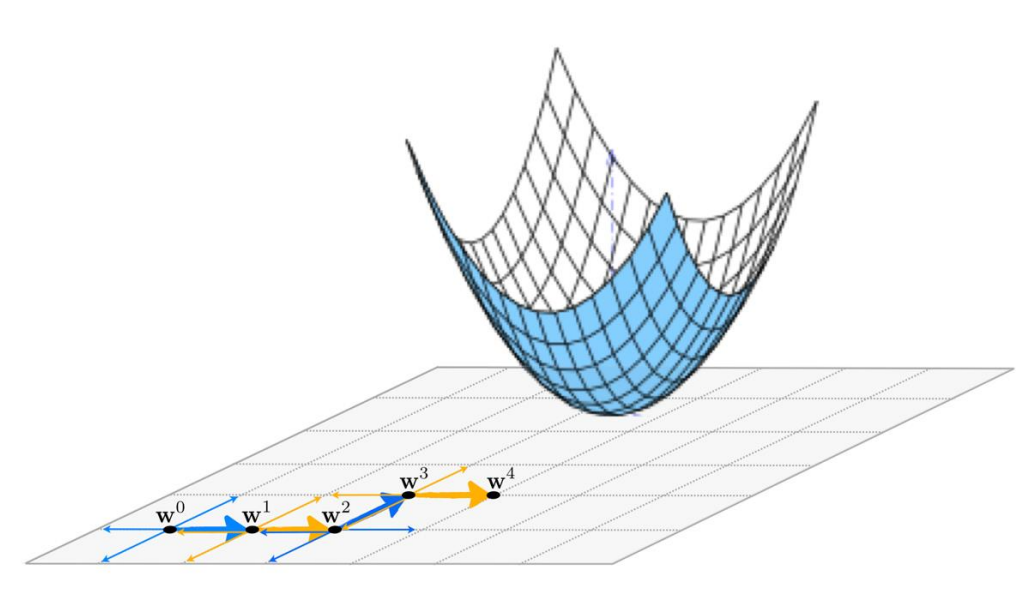
\includegraphics[width=0.4\textwidth]{img/lecture9/P5.png}
    \caption{Figure 9.4: Coordinate Search Algorithm: Exploring Descent Directions Along Coordinate Axes}
    \label{fig:P5.png}
\end{figure}


\section{Coordinate Descent}

While Coordinate Search explores directions without using gradients, Coordinate Descent improves efficiency by incorporating partial derivative information.

\subsection{Optimization}

Coordinate descent is an optimization strategy that improves the objective function by updating \textit{one parameter (one coordinate of $\vecb{\theta}$) at a time}. Instead of computing a full gradient vector across all parameters, the algorithm isolates a single coordinate direction and performs a one–dimensional optimization step along that axis. This greatly simplifies each update and reduces computational cost, especially in high–dimensional problems.

At each iteration, the algorithm selects a coordinate index \( j \in \{1,\dots,P\} \) and updates only the corresponding parameter while keeping all other parameters fixed. For a continuously differentiable loss function \(L(\vecb{\theta})\), the update rule becomes

\[
\theta_j^{t+1}
=
\theta_j^{t}
-\alpha \nabla_{\theta_j} L(\vecb{\theta}).
\]

This process is repeated across coordinates until convergence. The coordinates may be selected cyclically, randomly, or based on a heuristic such as the largest gradient magnitude. By decomposing a high–dimensional optimization problem into a sequence of simpler one–dimensional updates, coordinate descent can be particularly effective for large-scale machine learning problems where computing full gradients is expensive.

\begin{figure}[H]
    \centering
    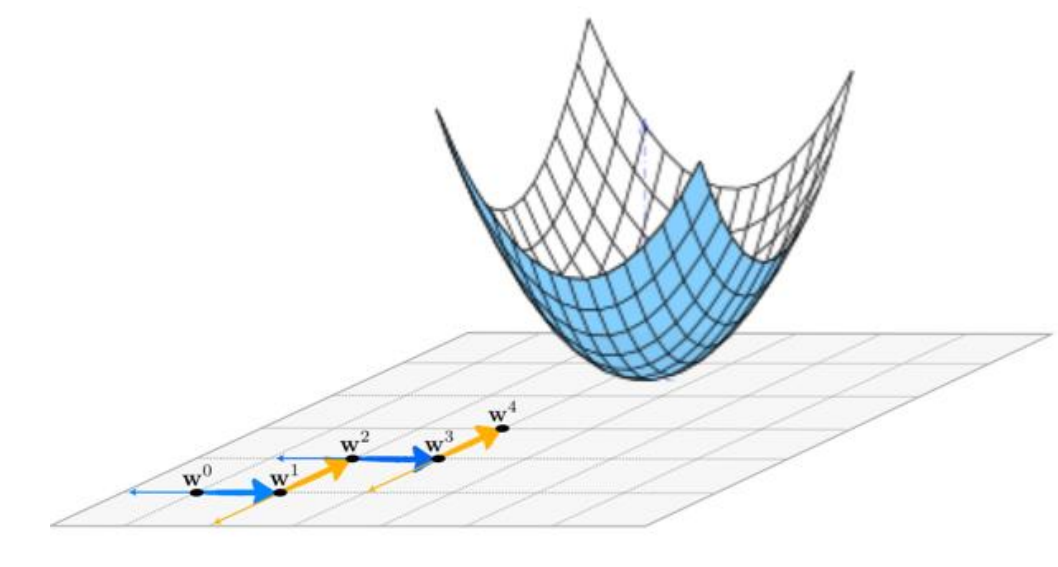
\includegraphics[width=0.4\textwidth]{img/lecture9/P6.png}
    \caption{Figure 9.5: Coordinate Descent Algorithm: Stepwise Optimization Along Coordinate Axes}
    \label{fig:P6.png}
\end{figure}

\subsection{Convergence}

In early iterations, coordinate search methods can make progress by exploring all coordinate directions, but coordinate descent quickly becomes more efficient once gradient information is used. Because each step directly follows the partial derivative with respect to a single parameter, the algorithm typically identifies descent directions faster and reduces the loss more effectively than coordinate search.

As illustrated in Figure~\ref{fig:P7.png}, coordinate descent tends to reach lower-cost regions of the objective function in fewer iterations. Although each step only adjusts one parameter, the repeated sequence of updates gradually drives the parameters toward a minimum. This stepwise progress often produces a characteristic ``zig-zag'' path toward the optimum.

\begin{figure}[H]
    \centering
    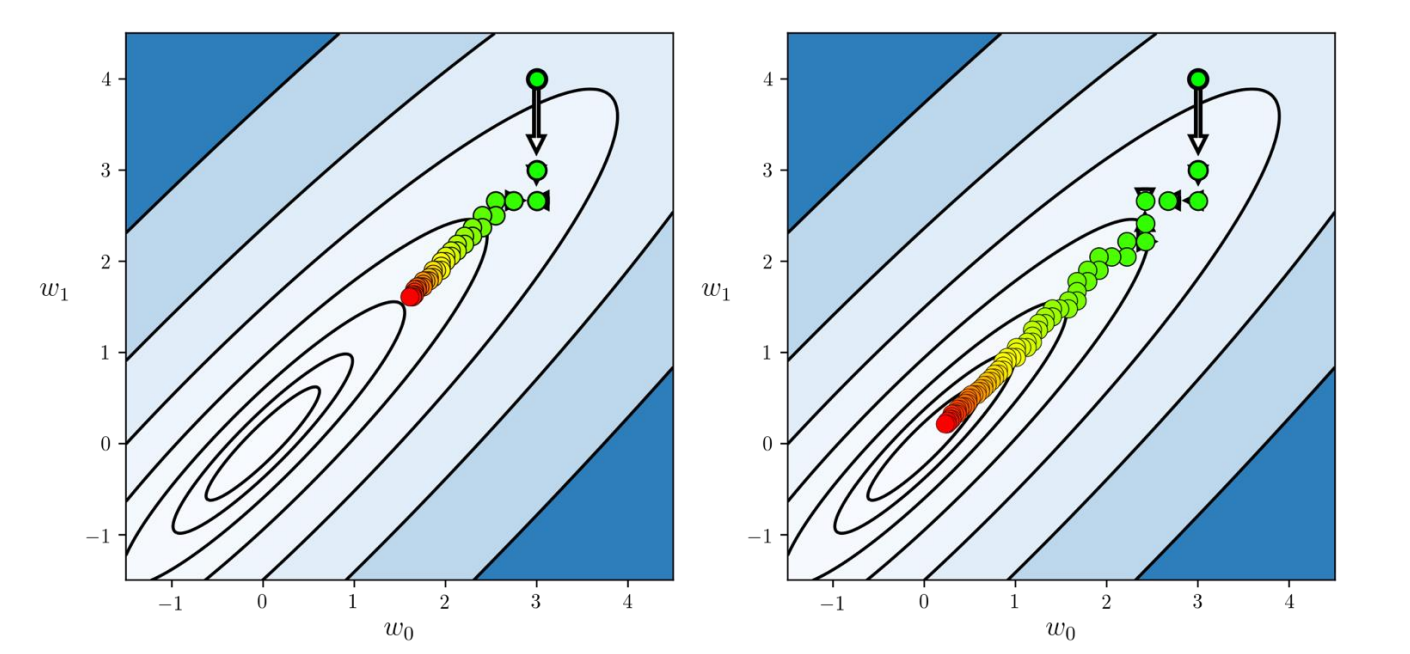
\includegraphics[width=0.4\textwidth]{img/lecture9/P7.png}
    \caption{Figure 9.6: Comparison of Coordinate Search (Left) and Coordinate Descent (Right): Efficiency in Finding Lower Cost Function Values}
    \label{fig:P7.png}
\end{figure}

\subsection{Advantages}

One of the main strengths of coordinate descent is its simplicity. Each update requires only a partial derivative with respect to a single parameter, making the method easy to implement and computationally inexpensive. Unlike second-order methods such as Newton's method, coordinate descent does not require storing or inverting large matrices, which makes it highly scalable to problems with many parameters.

Because of its low memory requirements and cheap updates, coordinate descent is widely used in large-scale machine learning applications such as Lasso regression, sparse optimization, and high-dimensional linear models.

\subsection{Limitations}

Despite its simplicity, coordinate descent has important limitations. The algorithm can struggle when the objective function is non-smooth or when variables are highly coupled. In such cases, improving one parameter at a time may lead to slow progress, oscillations, or convergence to suboptimal points such as saddle points.

Figure~\ref{fig:P8.png} illustrates an example of a non-smooth multivariable function. The sharp corners of the level curves make it difficult for the algorithm to determine a consistent descent direction. As a result, the optimization path (shown in red) can stall or progress very slowly toward the global minimum.

\begin{figure}[H]
    \centering
    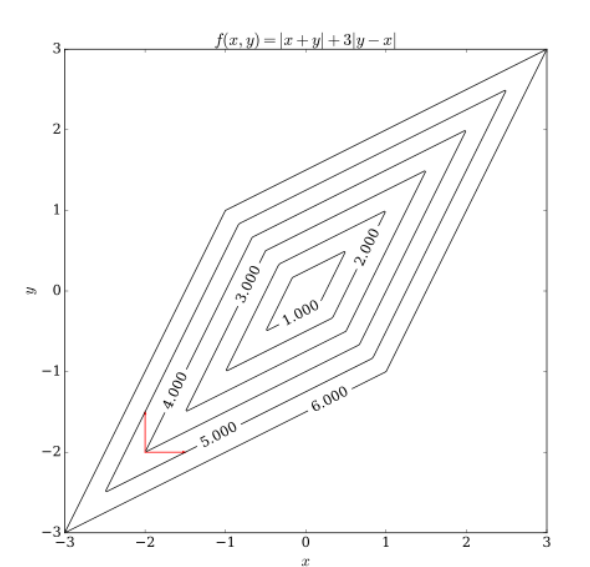
\includegraphics[width=0.4\textwidth]{img/lecture9/P8.png}
    \caption{Figure 9.7: A Case of Non-Smooth Multivariable Function}
    \label{fig:P8.png}
\end{figure}

The red trajectory highlights how the optimization may stagnate or move inefficiently due to the non-smooth geometry of the loss surface.



\section{Summary of Optimization Methods}

We now summarize the optimization methods discussed in Lecture 8 (first-order methods)
and Lecture 9 (second-order and coordinate-based methods).

\begin{table}[H]
\centering
\begin{tabular}{c|c|c|c}
\textbf{Method} & \textbf{Uses Gradient?} & \textbf{Uses Hessian?} & \textbf{Per–Iteration Cost} \\
\hline
Gradient Descent & Yes & No & Low \\
Newton’s Method & Yes & Yes & Very High ($O(P^3)$) \\
Coordinate Search & No & No & Medium \\
Coordinate Descent & Partial & No & Low \\
\end{tabular}
\caption{Comparison of Optimization Methods}
\end{table}

Each method presents a trade-off between computational cost and convergence speed. In practice, the choice of optimizer depends on the size of the dataset, the number of parameters, and the availability of derivative information.


% \section{Regularized Linear Models}

% \subsection{Overview}

% Regularized linear models extend ordinary linear regression by adding constraints that control the size of model parameters. In this lecture, we focus on three widely used regularization techniques: \textbf{Ridge Regression}, \textbf{Lasso Regression}, and \textbf{Elastic Net Regression}. Each method introduces a penalty term into the loss function that discourages overly complex models and helps improve generalization performance.

% \subsection{Motivation}

% Regularization is introduced to address a key limitation of standard linear regression: its tendency to overfit the training data when the model becomes too flexible. When a model overfits, it captures noise in the data rather than the true underlying relationship, which leads to poor performance on unseen data.

% Regularization techniques mitigate this issue by constraining the magnitude of the model’s coefficients. By penalizing large parameter values, the model becomes less sensitive to noise and more robust to variations in the training data. In practice, this results in simpler models that generalize better.

% There are several ways to impose such constraints on the coefficients of a linear model. The three most common approaches are Ridge Regression, which penalizes the squared magnitude of coefficients; Lasso Regression, which penalizes the absolute magnitude of coefficients; and Elastic Net Regression, which combines both penalties to balance their strengths.


\end{document}
